\documentclass{article}
\usepackage{graphicx} % for figures
\usepackage{float}
\usepackage[export]{adjustbox}
\usepackage{fancyhdr}
\begin{document}

\title{Physics 240 - Project report 3\\
		Roche surfaces}
\author{Tin Tran}

\maketitle

\section{Introduction}
This week is actually better as I finally got a contour plot to work, for the Earth and Moon. This would serve as a callibration for the upcoming sets of binary stars. 

\begin{figure}[H]
\centering{
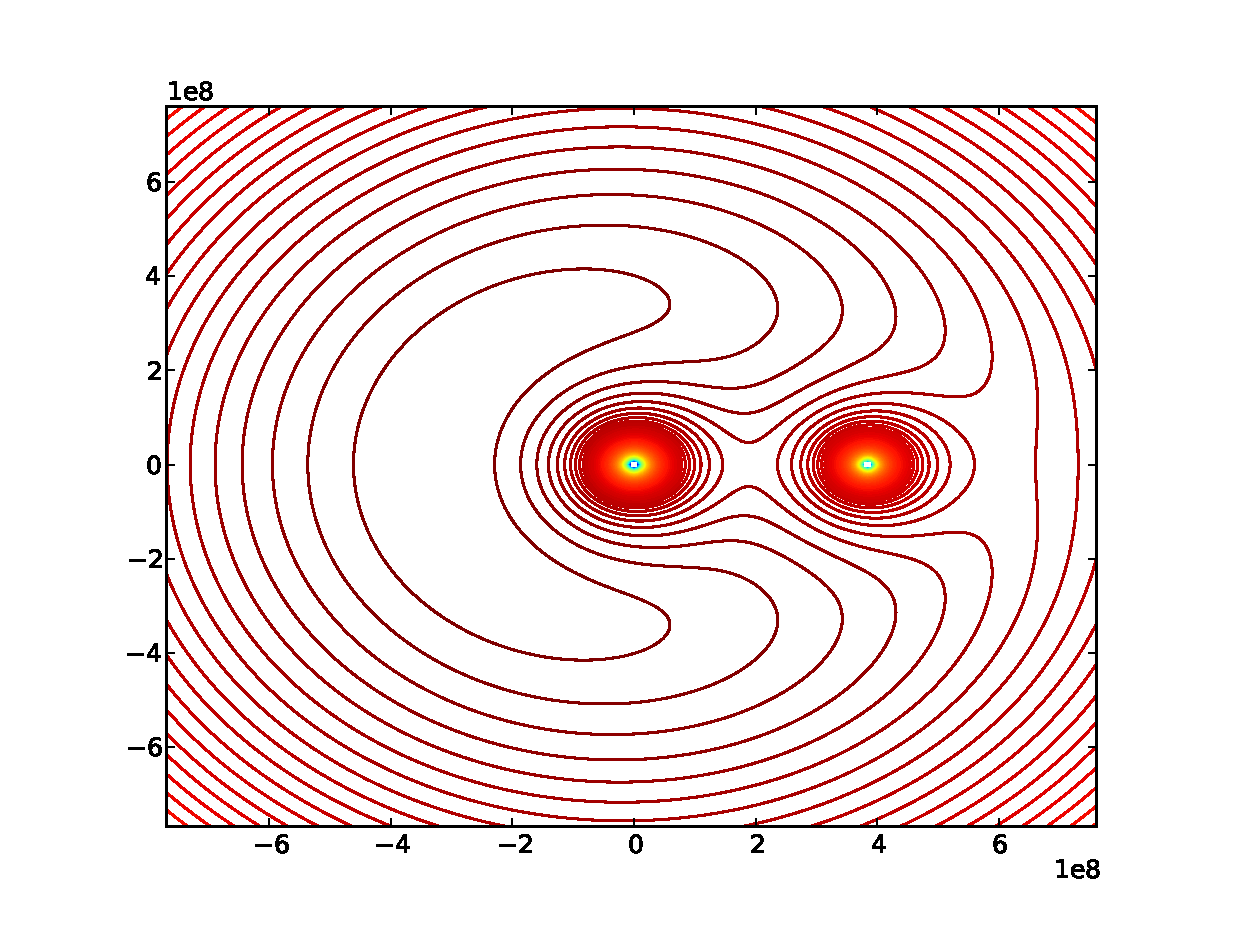
\includegraphics[max size={\textwidth}{\textheight}]{Contour2.eps}
\caption{Linear fit of Global Temperature vs time}
}
\end{figure}
As you can see on the plot, there are 2 Lagragian points, however there should be 5. So my next step is to adjust the contour level so that all 5 points should show up. The $\omega^2$ value could be what causing my problem here and I think once I have this sorted out, I can make more progress regarding different set of data and 3D plotting as well animations.\\
I also attached my current code as of now, and there's nothing much. I expect a lot more code to be written for the next report.

\end{document}